%%  File: main.tex
%%  Author: Matthew Gidden
%%  Created: Sept. 17, 2013
%%  Purpose: Prelim Presenation
     
\documentclass[10pt]{beamer}
\usetheme[white]{Wisconsin}
%\title[short title]{long title}
\title[Cyclus]{An Agent-Based Modeling Framework and Application for the Generic
  Nuclear Fuel Cycle}
%\subtitle[short subtitle]{long subtitle}
\subtitle[PhD Preliminary Examination]{PhD Preliminary Examination}
%\author[short name]{long name}
\author[MJG]{Matthew Gidden}
%\date[short date]{long date}
\date[09.23.2013]{September 23, 2013}
%\institution[short name]{long name}
\institute[UW-Madison]{University of Wisconsin-Madison}
% Page numbers.
\setbeamertemplate{footline}[page number]
% Those icons  in the references are terrible looking.
\setbeamertemplate{bibliography item}[text]
%try to get rid of header on title page\dots
\makeatletter
    \newenvironment{withoutheadline}{
        \setbeamertemplate{headline}[default]
        \def\beamer@entrycode{\vspace*{-\headheight}}
    }{}
\makeatother

% packages
\usepackage{multirow} % combining rows in tables
%\usepackage{footnote}

%% % this is a great way to compile only one (or more) frames at a time as you're
%% % working, saving tons on compile time
%% \includeonlyframes{current}

\begin{document}
%%%%%%%%%%%%%%%%%%%%%%%%%%%%%%%%%%%%%%%%%%%%%%%%%%%%%%%%%%%%%
%% From uw-beamer Here's a handy bit of code to place at 
%% the beginning of your presentation (after \begin{document}):
\newcommand*{\alphabet}{ABCDEFGHIJKLMNOPQRSTUVWXYZabcdefghijklmnopqrstuvwxyz}
\newlength{\highlightheight}
\newlength{\highlightdepth}
\newlength{\highlightmargin}
\setlength{\highlightmargin}{2pt}
\settoheight{\highlightheight}{\alphabet}
\settodepth{\highlightdepth}{\alphabet}
\addtolength{\highlightheight}{\highlightmargin}
\addtolength{\highlightdepth}{\highlightmargin}
\addtolength{\highlightheight}{\highlightdepth}
\newcommand*{\Highlight}{\rlap{\textcolor{HighlightBackground}{\rule[-\highlightdepth]{\linewidth}{\highlightheight}}}}
%%%%%%%%%%%%%%%%%%%%%%%%%%%%%%%%%%%%%%%%%%%%%%%%%%%%%%%%%%%%%

%% Cyclus/MJG Custom Commands
\newcommand{\Cyclus}{\textsc{Cyclus} }
%%%%%%%%%%%%%%%%%%%%%%%%%%%%%%%%%%%%%%%%%%%%%%%%%%%%%%%%%%%%%

%%--------------------------------%%
\begin{withoutheadline}
\frame{
  \titlepage
}
\end{withoutheadline}

%%--------------------------------%%
\AtBeginSection[]{
\begin{frame}
  \frametitle{Outline}
  \tableofcontents[currentsection]
\end{frame}
}
%---------------||||

%---------------||||
\section{Introduction}
\chapter{Introduction}\label{ch:intro}

\section{The Nuclear Fuel Cycle}

The nuclear fuel cycle can be described as a set of facilities that interact
with one another to either provide or consume fuel services. Facilities in the
fuel cycle act together to provide fuel to nuclear power plants which, in turn,
generate energy. The used fuel produced by the power plants is then returned to
servicing facilities to either recycle or dispose. The overall goal of the
system is to produce power at a competitive price while managing externalities
of the process, the chief of which is spent nuclear fuel. Myriad strategies
exist to achieve this aim which can be classified along a spectrum of the degree
to which fuel is recycled. In general, fuel cycles on the end of the spectrum
that does not recycle fuel are concerned most with cost, whereas fuel cycles
that fully recycle fuel are concerned most with issues of sustainability and
intergenerational equity. It is the goal of fuel cycle simulation to rigorously
explore this option space.

\subsection{The Open Fuel Cycle}

The open, or once-through, fuel cycle is relatively simplistic and is in place
in most countries in the world currently utilizing nuclear power. In practice,
the primary fuel element used in this type of cycle is uranium; however, a
combination of thorium and uranium, or some other initial source of neutrons,
could be used in theory. The fuel cycle is considered open because fuel that is
used in a reactor is stored indefinitely once its reactivity has dropped below
useful levels due to the presence of neutron poisons, primarily in the form of
fission products.

Uranium ore is initially extracted from the ground using one of a variety of
techniques including open pit mining, underground mining, and in situ
leaching. The uranium ore is then milled to form yellowcake,
$\mathrm{U_3O_8}$. The tailings, or byproducts, of this process are slightly
radioactive and are therefore considered to be low-level waste (LLW) by the
Nuclear Regulatory Commission (NRC) (see \citet{nrc_10_1985}). 

Certain reactors are designed to use naturally enriched uranium. For these
reactors, yellowcake can be directly reduced with oxygen to form naturally
enrich $\mathrm{UO_2}$. For the majority of power reactors, however, the uranium
must be enriched with higher-than-normal levels of uranium-235. In order to do
so, yellowcake is sent to a conversion facility, which converts it from
$\mathrm{U_3O_8}$ to $\mathrm{UF_6}$. The uranium hexaflouride is then enriched
to the required level in an enrichment facility, of which three classes exist:
gaseous diffusion, the original enrichment technology; centrifugal diffusion,
the current enrichment technology; and Atomic Vapor Laser Isotope Separation
(AVLIS), a newer technology not currently in commerical production. The enriched
uranium hexaflouride is then sent to a fuel fabrication facility where it is
returned to yellowcake form before being reduced to uranium oxide, similarly to
the process for natural uranium fuel. The uranium oxide is then sintered into
pellets and loaded into fuel assemblies to be placed in a reactor. This process
in conjunction with uranium mining is termed the 'front end' of the nuclear fuel
cycle.

Making the open fuel cycle unique, once fuel has been processed in a reactor, it
is cooled off in pools for a number of years, and then stored in dry casks
before eventually being sent to a final repository. The physical location of the
fuel may vary during dry cask storage between the reactor site or some other
interim storage site.

Graphically, the open fuel cycle is shown in Figure \ref{fig:open-cycle}.

\begin{figure}[]
  \begin{center}
    \includegraphics[width=6cm]{./chapters/intro/open_cycle.png}
  \caption{The once-through fuel cycle as shown in \cite{cochran1990nuclear}.}
  \label{fig:open-cycle}
  \end{center}
\end{figure}


\subsection{The Closed Fuel Cycle}
The closed fuel cycle is one that includes the recycling of used, or spent, fuel
to be reused in a reactor. Spent fuel that exists the average Light Water
Reactor (LWR) has an elemental makeup shown in Table \ref{tab:lwr_fuel}. The
economics of recycling spent fuel is complicated and depends on many external
factors, but doing so has two overarching benefits that contribute to lowering
the cost of the fuel cycle: increasing repository capacity and increasing fuel
utilization. 

\begin{table} [h]
\centering
\begin{tabular} {|c|c|} 
\hline
Element Group & wt \% \\
\hline
Uranium           & $\mathrm{\sim}$95  \\
Plutonium         & $\mathrm{\sim}$1   \\
Mixed Actinides   & $\mathrm{\sim}$0.1 \\
Fission Products  & $\mathrm{\sim}$4   \\
\hline
\end{tabular}
\caption{Elemental Breakdown of Spent Fuel Exiting a Typical LWR}
\label{tab:lwr_fuel}
\end{table}

Of the elements that comprise used fuel, uranium, plutonium, and the mixed
actinides (MA) are all capable of producing power through the fission
process. The fission products, however, contain isotopes with high neutron
capture cross sections, which therefore act as poisons to the nuclear chain
reaction.  Achieving 100\% fuel utilization would thus require storing
indefinitely only the fission products and any other byproducts of the fuel
cycle. Furthermore, repository capacity is determined not necessarily by total
mass, but rather by heat load and radiotoxicity, making the concentration of
high-activity isotopes the limiting factor in a repository's capacity. Fission
products are generally short-lived (in comparison to transuranic elements, i.e.,
uranium, plutonium, and the MAs). Accordingly, by minimizing the amount of
transuranics in a repository, its capacity can be extended.

The act of reprocessing spent fuel is a requires relatively few steps. Once fuel
has left the reactor core, it is stored in a spent fuel pool for a some number
of years, typically around five. It can then be directly sent to a reprocessing
facility or be sent after some period of dry-cask storage. Reprocessing fuel is
a chemical extraction process and therefore is limited by chemical extraction
techniques. In general, there are two types of such processes: low-temperature
methods using organic solvents (e.g. PUREX), and high-temperature methods using
molten salts and metals, called pyroprocessing. The extraction techniques
separate the spent fuel into chemically-similar groups which can be different
based on the technique used. However, the separated groups are usually some
combination of those shown in Table \ref{tab:lwr_fuel}. The separated streams
are then sent either to a repository as high-level waste (HLW) or to an
appropriate fuel fabrication facility. Graphically, the closed fuel cycle is
shown in Figure \ref{fig:closed-cycle}.

\begin{figure}[]
  \begin{center}
    \includegraphics[height=7.5cm]{./chapters/intro/closed_cycle.png}
  \caption{The closed fuel cycle as shown in \cite{cochran1990nuclear}.}
  \label{fig:closed-cycle}
  \end{center}
\end{figure}


The elemental groups used in fuel fabrication will depend on the fuel cycle that
is developed. The only large-scale industrial reprocessing plants (La Hague in
France, THORP in the U.K., Mayak in Russia, and Rokkasho in Japan) utilize the
PUREX process to extract uranium and plutonium. The plutonium is then oxidized
and mixed with depleted Uranium from the enrichment process to produce what is
known as mixed-oxide fuel (MOX). Other sources of uranium can be used to fill
MOX fuel, as neutronics-related reactivity and safety constraints allow. Other
fuel cycles utilize the mixed actinides elemental group as well. These generally
include fast reactors that convert their transuranics inventory into either more
TRU (i.e., they have a conversion ratio (CR) of greater than 1), less TRU (CR <
1), or they maintain the amount of TRU entering and exiting their system (CR =
1). Fast reactors with CR > 1 are called breeder reactors.

It should be noted that with any reprocessing capability, nonproliferation
issues arise. Nuclear weapons have historically been produced using either
enriched uranium or plutonium; however it is possible to produce one with any
mix of appropriate materials. Accordingly, any fuel cycle that exposes bare
plutonium streams has an inherently higher nonproliferation risk than one that
does not, and such risks must be weighed accordingly. On a technical note,
though, the relatively low content of Pu-239, especially with respect to the
concentration of heat-producing Pu-240, in spent LWR fuel makes diverting such
fuel for the purposes of nuclear weaponry a route with a near-non-existant
probability of success.


\subsection{The Modified-Open Fuel Cycle}
The modified open fuel cycle is effectively a hybrid of the open and closed fuel
cycles. The Blue Ribbon Commission's Reactor and Fuel Cycle
Technology Subcommittee tackled a definition as follows:

\begin{quotation}
We have defined this category to encompass a very wide range of possible fuel
cycles with multiple possible combinations of different reactor, separations,
and fuel fabrication technologies. Our definition includes any fuel cycle in
which some of the spent fuel is processed rather than being directly disposed of
after a single pass through a reactor.~\cite{brc_reactor_2012}
\end{quotation}

They mention, however, that there is no industry-wide agreed-upon
definition. For the purposes of this work I will use the committee's
definition. It should be noted that by the committee's definition, the French
nuclear power program is technically a modified-open cycle because MOX fuel
reprocessing has been demonstrated, but is not used at an industrial scale.


\section{Fuel Cycle Simulation}

\subsection{Overview}\label{sec:simulators-overview}
Fuel cycle simulation is a field with a variety of actors. The majority are
state-base (i.e., part of a government's national R\&D infrastructure), but
other players include universities as well as international governance
organizations such as the International Atomic Energy Agency (IAEA). The
modeling strategies applied to the nuclear fuel cycle span a wide range of
fidelity, both at the facility level and the material level. For instance, some
simulators describe reactors by fleet (or types) and solve material balances for
the entire fleet in aggregate while others instantiate individual (or discrete)
facilities. Similarly, some simulators make detailed calculations of fuel
depletion due to reactor fluence whereas others simply use pre-tabulated values
that depend (generally) on burnup values for thermal reactors and conversion
ratios for fast reactors.

There are, broadly, three decision categories that are of concern to fuel cycle
simulation. The first is facility deployment, specifically, how and why certain
facilities are deployed. There is general consensus regarding reactor deployment
in the community: a user defines an energy growth curve and, for each type of
reactor in the simulation, a percentage of that total energy demand to be met by
the reactor type. However, the nuclear fuel cycle is a special case of
supply-demand modeling where certain facilities (e.g., fast reactors) require
fuel that has been processed by other facilities (e.g., thermal
reactors). Accordingly, simulation developers must make a choice: should one
allow a facility to be built if it may not be able to be fueled? Certain
simulators explicitly disallow this behavior by determining reactor build
decisions based on lookahead algorithms (e.g., CAFCA, VISION), others explicitly
allow it (e.g., COSI), while still others offer a hybrid approach that allow a
lookahead function based on a certain amount of fuel that will eventually be
needed over a reactors lifetime (e.g., DANESS). The eventual choice of this
decision making process greatly affects simulation outcomes in any scenario in
which a lack of fuel exists. Because these simulation tools are built to analyze
the dynamic symbiotic relationship between different reactors in a cyclical
process (e.g., thermal and fast reactors), among other scenarios, this
simulation development decision is arguably very important to simulation
outcomes.

The second major simulation development decision is determining fuel
isotopics. A number of complications are encompassed in this decision. As an
example, consider MOX fuel for thermal reactors. In general, MOX fuel is
composed of oxide forms of plutonium (and some minor actinides, such as
americium) from spent thermal fuel as well as uranium (the source of which can
be depleted enrichment tails, depleted recycled uranium or natural uranium). The
fact that depleted uranium, rather than enriched uranium, can be used stems from
the fact that the separated plutonium is largely comprised of fissile isotopes
(\nucl{239}{Pu} and \nucl{241}{Pu}). The source of uranium already introduces an
isotopic dependency of importance: the \nucl{235}{U} enrichment of the fill
uranium should affect either the quantity of plutonium used, the isotopics of
plutonium used (with higher \nucl{235}{U} enrichment implying a lower
concentration of fissile plutonium isotopes), or both. Further complicating the
issue is that plutonium isotopes are radioactive and decay on (relatively) short
time scales. For instance, the half life of \nucl{241}{Pu} is $\sim$14
years. Accordingly, the quality, or isotopic content, of the separated plutonium
changes on a time scale on the order of the simulation due to decay. There is a
similar issue with other transuranic radioactive isotopes of interest to nuclear
fuel cycles.

Accordingly, simulation developers have two general choices with respect to
input fuel isotopics (and isotopic-level modeling in general). The first is
whether or not to include isotope decay. As might be expected, the simulators
fall into two camps, those that include decay (e.g., VISION and COSI) and those
that do not (e.g., DANESS and CAFCA). Interestingly, the MIT development team
claims that the lack of modeling decay does not affect the simulation as long as
all transuranic isotopes are lumped together \cite{guerin_impact_2009}. Other
codes appear to include isotopic decay in order to inform output metrics such as
repository heat capacity. The second choice involves matching input isotopics
with available separated isotopes. This is an interesting problem because
separations technology work on a elemental scale, whereas input fuel recipes are
defined on an isotopic scale because neutronics properties are functions of
individual isotopes rather than elemental aggregates. In other words, you can't
change the separated plutonium isotopic vector to match a recipe, as one does
with uranium enrichment (which is an isotopic-scale process). A full treatment
of the problem is relatively complicated and requires mixing separated plutonium
vectors to find a ``best match''; this problem has been termed the Winery
Problem or the Recipe Approximation Problem \cite{oliver_geniusv2:_2009}. The
current generation of fuel cycle simulators generally punt on this issue. A
common strategy is to declare a target subset of isotopics, normally a specific
plutonium isotope or the aggregate plutonium isotopes, and match quantities of
that set. For example, if the set is of single cardinality (e.g.,
\nucl{239}{Pu}), then the amount of that isotope is guaranteed to be correct,
but accompanying isotopics are not. On the other hand, if the set is a group of
isotopes (e.g., all plutonium isotopes), that group's quantity is guaranteed to
be correct, but the specific isotopics are not. One can conclude from this
discussion that the level of isotopic detail modeling in a simulation could
greatly affect the outcome of the simulation, especially if decisions are made
mid-simulation regarding the isotopes in question (e.g., whether or not to build
a fast reactor given the available amount of separated isotopes). A full
treatment of how the current generation of simulators tackle this issue is
described in \S\ref{sec:simulators}. An overview of the proposed strategy to
take in the \Cyclus simulation environment is described in \S\ref{sec:rap}.

The third major development decision is how to determine connections between
facilities. At issue here is how servicing facilities (e.g., fuel fabrication
facilities) are connected to serviced facilities (e.g., reactors). For those
simulators that do not model discrete facilities (e.g., CAFCA), the modeling
technique is relatively trivial: a fleet of servicing facilities are directly
connected to their serviced facilities. If more than one type of facility is
being serviced (e.g., TRU-based fuels going to thermal and fast reactors), then
a user must define the percentage of capacity going towards each type of
serviced facility \cite{busquim_e_silva_system_2008}. A similar situation arises
in other systems-dynamics based simulators, because mass flow balance equations
govern the inner workings of the simulations. This situation becomes even more
complicated if regional scenarios are to be modeled. In addition to determining
which serviced facilities will be connected to servicing facilities, one must
also incorporate a notion of the region of serviced and servicing
facilities. DESAE includes a rather simplistic model of this relational nature
that predetermines the yearly intra-regional trading \cite{iaea_nuclear_2010}. A
full treatment of this class of developmental decision making with respect to
the current set of fuel cycle simulators is provided in
\S\ref{sec:simulators}. An overview of the proposed strategy to take in the
\Cyclus simulation environment is described in \S\ref{sec:rap}.


\subsection{Metrics}
Fuel cycle simulators have a number of possible output metrics of interest. One
of the original reasons that fuel cycle simulators were developed was to
determine the relative cost of different fuel cycles. This is also a key example
of differences between simulators. The notion of fuel cycle cost can either be
calculated in a post-processing step, or it can be calculated on-the-fly during
a simulation. The benefit of maintaining cost information during a simulation is
that the simulation can react to these costs. A prime example of such behavior
is in the DANESS simulation code, described in \S\ref{sec:other-sims}. 

A large number of metrics related to fuel cycle simulation come directly from
the material mass flows. For instance, proliferation based metrics are generally
determined by the amount of separated transuranic material at any point in the
fuel cycle. Metrics that lead to less proliferation resistance include the
amount of signifigant quantities of material, defined by the IAEA to be the
quantity of any given material (e.g. TRU or plutonium) sufficient to make a
nuclear weapon. These are generally defined on the elemental level, which
ignores realities based on isotopic dependencies (e.g. \nucl{240}{Pu} is a
relatively large source of decay heat and is thus reduces the aggregate
plutonium's effectiveness for use as a weapon). Metrics that lead to more
resistance of proliferation activities include the unshielded dose rate of a
given material, which makes handling (and thus diverting) the material more
difficult \cite{yacout_vision_2006}. Another key metric that is important to
many in the fuel cycle simulation community is uranium utilization. At present,
the United States political stance is to continue the once-through fuel cycle
until it is economically viable to begin reprocessing spent fuel for recycle in
reactors \cite{hamilton_blue_2012}. Such a situation can only arise if the
supply of uranium dwindles to a low-enough level which will raise the price of
uranium sufficiently enough to make reprocessing a viable alternative. It is
additionally interesting to note the approximate time at which uranium capture
from seawater, which is in developmental stages, will become economically
viable. These situations all depend on the amount of uranium used in a given
simulation, which is, of course, related to fuel mass flows.

One of the key outputs of simulators is related to repository capacities. The
capacity a repository to store spent fuel could be reached in a number of
ways. Spent fuel isotopics, especially fission products, produce a large amount
of decay heat which can reach the thermal limits of their containers over short
periods of (geologic) time. There are also radiotoxity limits for repositories
in order to limit the risk of radiological releases. Finally, there is a mass
and volume limit on repositories, representing a space storage capacity. It is
not clear at the current time which of these limiting capacities will
ultimiately be the governing factor for repositories. Furthermore these
capacities change based on repository layout and geology. A more in-depth study
is presented by Katy Huff in her thesis work
\cite{huff_integrated_2013}. Furthermore, this parameter was key in Scopatz's
work with static fuel cycle simulation \cite{scopatz_essential_2011}. In all
cases, these capacities can be calculated in terms of isotopic quantities of
waste products. It is possible to calculate the capacity parameters \textit{in
  situ} during the simulation and dynamically alter the simulation based on the
results rather than simply performing a post-processing operation to report the
required number of repositories for the simulation. 


\subsection{Benchmarks}\label{sec:intro-benchmarks}
The effort to benchmark fuel cycle simulation codes has occured (relatively)
recently, and there have been a number of different benchmarking exercises
attempted by governmental and international agencies to date. The most notable
of these are the International Atomic Energy Agency (IAEA) International Project
on Nuclear Reactors and Fuel Cycle's (INPRO) benchmark
exercise \cite{_international_2009}, the Massachusettes Institute of
-Technology's benchmark exercise \cite{guerin_benchmark_2009}, the Nuclear Waste
Technology Review Board's (NWTRB) benchmark
exercise \cite{abkowitz_workshop_2011,_nuclear_2011} and the Organization for
Economic Cooperation and Development's (OECD) benchmark
exercise \cite{boucher_benchmark_2012}.

Each of the benchmarking efforts used a different set of codes by which to
compare agaisnt one another. The codes used in each is described in
Table \ref{tab:benchmark-codes}.

\begin{table} [h!]
\centering
\begin{tabular} {|c|c|} 
\hline
Benchmark & Codes Used \\
\hline
IAEA - INPRO & COSI, DESAE, FAMILY, TAPS, VISTA, VISION \\
MIT          & CAFCA, COSI, DANESS, VISION \\
NWTRB        & AREVA, CAFCA, NUWASTE, VISION \\
OECD         & COSI, EVOLCODE, DESAE, FAMILY, VISION \\
\hline
\end{tabular}
\caption{The Set of Codes Compared in Each Benchmarking Effort}
\label{tab:benchmark-codes}
\end{table}

Each benchmarking effort investigated a different set of scenarios. The actual
scenarios investigate depends heavily on the interest of the organizing
institution. For example, the NWTRB is a congressionally mandated review board,
thus their scenario suite focused on options for the U.S. fleet of nuclear
reactors. The INPRO benchmarks called for scenarios with low, moderate, and high
nuclear power capacity growth. For each growth scenario, three different
deployment scenarios were modeled: PWRs and HWRs; PWRs, HWRs, and advanced PWRs;
and PWRs, HWRs, advanced PWRs, and fast reactors. The actual specifications for
reactor power level, fuel isotopic composition, and any other simulation
parameters (outside of the power level and types of reactors to be used) were
provided in a reference database \cite{_international_2009}. The MIT benchmark
incorporated the growth of nuclear power demand in three categories: 0 \% per
year, 1.5 \% per year, and 3 \% per year, all of which are rates of exponential
demand growth. The deployment schemes include: LWRs fueled with UOX
transitioning to fast reactors with conversion rates of 0.5, LWRs with UOX and
(eventually) MOX transitioning to fast reactors with conversion rates of 0.5,
and LWRs fueled with UOX transitioning to fast reactors with conversion rates of
1.0. The transition period began at year 2040 in each scenario. This set of
specifications is tailored to be easily met by the host institution's simulation
code, CAFCA (see \cite{guerin_benchmark_2009} and \S\ref{sec:cafca}). The NWTRB
benchmark breaks scenarios down into
``phases'' \cite{abkowitz_scenario_2011}. The first phase is a starting point,
representing spent fuel currently in the system. The second phase models a
constant power level held at the 2009 level (100.3 GWe), with new plants coming
online to keep that power level constant when older reactors retire. The third
phase models a scenario in which a repository opens in year 2040 and includes a
constraint on the age of fuel that can enter the repository. The fourth phase
models a suite of scenarios in which a reprocessing facility enters operation at
year 2040. The family of scenarios varies the separations capacity from 1500 to
3000 t/yr and varies the allowable fuel age from 5 to 50 years. The fifth phase
models scenarios that incorporate both reprocessing and a repository. The OECD
benchmark assumes a constant installed power for each scenario with reactor
deployments varying across scenarios. The first scenario assumes an open cycle,
i.e., power is only met by PWRs using UOX fuel. The second scenario assumes that
some percentage of the PWRs can use MOX fuel. The third scenario assumes that
for a finite period of time, MOX is used by some LWRs, and after 80 years, all
retired LWRs are replaced by fast reactors.


discuss how the scenarios were described, citing boucher as the best

It must be noted that the fuel cycle simulation community does not benefit from
benchmarking exercises in the same way that the nuclear physics community
benefits from them. For example, the Monte Carlo N-Particle (MCNP) code
community has a number of criticality safety benchmarks \cite{wagner_mcnp:_1992}
which have been verified by years of experiment and experience. Put another way,
for certain MCNP problems, there is a \textit{verifiably correct answer}. The
community can then build up from those basic principles to understand how
``believable'' their solutions are for larger, more complex problems. This is,
in fact, the reason why benchmarks exist. Fuel cycle simulation does not
necessarily have these characteristics. For instance, there is a fundamental
difference between simulations that model continuous material flow versus those
that model distcrete material transfers. Accordingly there is no ``right
answer'' for even most simple simulations. Instead, there must be a community
consensus, which leads to benchmarking exercises that incorporate some subset of
the simulators in the community. In general, these exercises compare large,
aggregate metrics in order to limit differences caused by fundamental
differences in modeling approaches. For example, benchmarks may compare the
total aggregate flow of used fuel coming out of reactors. However, one can't
really come to a consensus answer regarding the isotopics of this spent fuel due
to the wide variety of simulator treatment of depletion and decay (ranging from
no use of such methods to full integration of depletion codes).

In his conclusions of the MIT benchmarking exercise, Guerin states that
``operation of a fuel cycle model is as much art as science''
\cite{guerin_benchmark_2009}. Understanding just how much of FCS is art and how
much is science is critical to providing reliable results. 


\section{Open Questions in Fuel Cycle Simulation}
\subsection{Using Agent-Based Models}

Stepping back a moment from the discussion of nuclear-specific fuel cycles, the
interactions that we wish to model are those of supply and demand. Certain
facilities need some sort or raw or processed material that other facilities
produce. The fuel cycle is more complicated than this simple statement, though,
because facilities are connected through recycled fuel. Even with such a
complication, the notion of a generic fuel cycle, i.e. from the perspective of
facilities that supply and demand material, quickly begins to look like a supply
chain model. There is a growing literature of agent-based supply chain modeling
\cite{swaminathan_modeling_1998,julka_agent-based_2002,van_der_zee_modeling_2005,chatfield_multi-formalism_2007,holmgren_agent_2007}.
The general premise of these types of models is that individual facilities have
a notion of their needs (i.e., their demands) and can express to the system
these needs at the required time. There is heavy use of inventory policy to
determine the correct amount of material inventory that is needed and the
correct time to request a resupply. In general, a facility may be comprised of
many agents, e.g. an ordering agent, a stocking agent, a forecasting agent,
etc. Such an approach has not heretofore been attempted for the nuclear fuel
cycle and opens up a variety of doors. For example, reactor facilities could be
allowed to be fueled by multiple fuel types (e.g., UOX or MOX), and decide which
type to choose based on the simulation environment. However, due to the
fungibility of material in the fuel cycle (plutonium, for instance, can be used
by fast reactors and thermal reactors), many questions remain about how to
describe the materials to be traded and the markets on which they will be
traded. A more fully formed proposal for such a treatment is presented in
\S\ref{sec:gfctp}.

\subsection{Input Fuel Isotopic Matching}

One of the major issues with current fuel cycle simulation is the disconnect
between fuel recipes being requested by reactors that need recycled fuel,
e.g. MOX fuel. The isotopics that comprise these materials, especially the
transuranic isotopes, are radioactive, and thus the actual isotopic composition
of material change with time. Accordingly, if a simulator wishes to try to match
the requested isotopics, it must keep track of the decay of isotopes. Further
complicating the problem is that requested input fuel recipes may not
necessarily be related to the provided output fuels, i.e., there is a mismatch
between the output isotopics and input isotopics even without the presence of
isotopic decay. The majority of fuel cycle simulators to date ignore this issue
and instead choose to match recipes ``exactly'' based on a subset of
isotopes. Further details of how other simulators tackle this issue are reviewed
in \S\ref{sec:simulators}. A full treatment of the recipe-matching problem would
require an approach similar to the pooling-blending problem
\cite{tawarmalani_convexification_2002}. There is a rich literature base for
pooling-blending problems
\cite{glen_mixed_1988,rigby_evolution_1995,mendez_simultaneous_2006,misener_advances_2009}
in the industrial processes literature. However, the majority of the subject
matter concentrates on refinery operations such as mixing various crude oils to
hit a certain octane level. These are (relatively) simple problems because the
properties that are trying to be matched are extrinsic and linear function of
the mixing variables. The nuclear arena is much more complicated because of
criticality limitations and the want to match aggregate nuclear properties of
materials. Accordingly, a hybrid approach was proposed that involves blending and
approximation theory. The approach is outlined in \S\ref{sec:rap}.

\subsection{Modeling Global Regions}

The notion of regional modeling in fuel cycle simulation has always been a
secondary concern. Certain simulators attempt to model it explicitly, e.g. DESAE
\cite{iaea_nuclear_2010}. Other simulators have attempted to add the capability
at some point after their simulator had already been developed, e.g. VISION and
COSI. A discussion of these capabilities follows in \S\ref{sec:simulators}. Some
semblance of this capability is needed if one is to incorporate outside effects
on a domestic fuel cycle. Furthermore, a robust capability is required if one
wishes to actually investigate dynamic interactions amongst regional
entities. Again, a full treatment of this sort of regional interaction would
require international relations models, most of which can be found in the
cross-cutting realm of economics, political science, and game theory. The
primary solution technique is called Nash Equilibrium, and effectively describes
an optimal solution as follows: given a set of players, states, preferences,
and actions, all players choose an action such that any single player's
deviation from that actions results in a state of lower preference for that
player (thus no player has an incentive to deviate)
\cite{mccarty_political_2007}. There also exists a body of literature that
examine Nash Equilibria in the context of optimal flow models
\cite{mazumdar_fairness_1991,nagurney_supply_2002,song_nash_2002}. However, the
complexity of such models quickly brings them out of the scope of our needs,
i.e., dynamic modeling of multi-lateral scenarios ranging 100+ years in a
short-time ($\sim$2-5 minutes). Accordingly, a market resolution mechanism has
been proposed that allows for interaction amongst the various facilities and
managing entities (e.g. their regions). In order to inform a cardinal preference
\cite{strotz_cardinal_1953} relation for a facility over its possible supply
materials. The full approach is outlined in sections \S\ref{sec:gfctp} and
\S\ref{sec:agent-interaction}.


\section{Fuel Cycle Simulation}
% simulation.tex

\begin{frame}[ctb!]
  \frametitle{Simulating the Nuclear Fuel Cycle} 

  Fuel cycle simulators are designed to answer policy-related questions
  regarding transitions from one equilibrium state to another.

  \vspace{0.2cm}

  \pause
  A simulator answers the following questions as a function of its 
  parameter space:
  \begin{itemize}
    \item how much material exists
    \item where does that material reside
    \item from/to where and when is material transported
    \item what kinds of facilities are needed
    \item when is each type of facility needed
  \end{itemize}
\end{frame}

\begin{frame}[ctb!]
  \frametitle{Simulating the Nuclear Fuel Cycle}
  The nuclear fuel cycle is simulated via \textit{scenarios}.\vspace{0.2cm}

  A scenario generally defines a demand for nuclear power and the types of
  reactors that can respond to that demand. Supporting facilities can be
  explicitly or implicitly modeled to provide fuel for the reactors, and such
  behavior depends on the model used by the simulator.\vspace{0.2cm}

  Some nuclear fuel cycle simulators (FCS) currently in use today:
  \begin{itemize}
    \item CAFCA (MIT) \cite{busquim_e_silva_system_2008}
    \item COSI (CEA) \cite{boucher_cosi:_2006}
    \item DANESS (ANL) \cite{durpel_daness_2003}
    \item VISION (INL) \cite{yacout_vision_2006}
  \end{itemize}
\end{frame}

\begin{frame}[ctb!]
  \frametitle{FCS Metrics}

  FCSs generally report back metrics about the fuel cycle in question. Many of
  these metrics are functions of facility deployment, material flow, and
  material residency, including:

  \begin{itemize}
    \item economics
    \item waste management
    \item sustainability
    \item nonproliferation
  \end{itemize}
\end{frame}

\begin{frame}[ctb!]
  \frametitle{FCS Design Choices}
  Simulation designers are faced with a number of decisions, including:
  \begin{itemize}
    \item facility deployment
    \item fidelity of physical, chemical, and industrial processes
    \item material transaction modeling
  \end{itemize}
\end{frame}

\begin{frame}[ctb!]
  \frametitle{FCS Design Choices: Deployment}

  Reactor deployment choices in almost all cases are chosen by the user.\vspace{0.2cm}

  Supporting facility deployment can be chosen by the user, but in most present
  cases, they are deployed when needed by a look-ahead function.\vspace{0.2cm}

  In many present cases, deployment, although user defined, is restricted by
  future available material. For example, if an advanced reactor requires
  transuranic (TRU) fuel, and a simulation knows that TRU will not be available,
  simulators instead deploy a non-constrained reactor.\vspace{0.2cm}

  In such cases, a class of reactors, e.g. LWRs, is considered never to be
  fuel constrained.
\end{frame}

\begin{frame}[ctb!]
  \frametitle{FCS Design Choices: Fidelity}

  Physical, chemical, and process fidelity are all design choices for simulators.\vspace{0.2cm}

  Physical fidelity includes the choice to model isotopic decay and whether or
  not to model in-core reactor physics.\vspace{0.2cm}

  Chemical and process fidelity include the modeling of the chemical separations
  and advanced fuel fabrication processes. The separations-fuel fabrication
  interface is generally not treated by the current simulator cadre.
\end{frame}

\begin{frame}[ctb!]
  \frametitle{FCS Design Choices: Material Transactions}

  Determining how material flows, or is transacted, is a critical design
  decision, because of the effect it has on output metrics.\vspace{0.2cm}
  
  Most simulators in use to date use a systems dynamics approach, which models
  aggregate material flows between fleets of reactors.\vspace{0.2cm}

  These flows are \textit{static}, i.e., connections between fleets of
  facilities are known \textit{apriori}. In fact, these connections govern the
  equations used in the systems dynamics modeling architecture. This makes
  extensibility of the codes difficult for any new type of fuel cycle.
\end{frame}

\begin{frame}[ctb!]
  \frametitle{FCS Design Choices: Summary}
  
    \begin{table} [h!]
      \small
      \centering
      \begin{tabular} {|c|c|c|c|c|}
        \hline
        Decision                     & Category & CAFCA & COSI & VISION \\ 
        \hline
        \multirow{2}{*}{Deployment}  & Determined by 
        & user & user & user \\ \cline{2-5}
        & Constrained by\footnote{Generally a look-ahead function determines the associated metric.}   
        & available material & not treated by literature & available material \\ \hline
        \multirow{3}{*}{Fidelity}    & Decay 
        & yes\footnote{Capability is available, but it is not used.} & yes & yes \\ \cline{2-5}
        & Reactor Physics 
        & no & yes & no \\ \cline{2-5}
        & Fuel Matching\footnote{How recycled fuel orders are ``matched'' with available isotopics.} 
        & aggregate mass flows & equivalence method & aggregate mass flows \\ \hline
        \multirow{2}{*}{Connections} & Static/Dynamic 
        & static & static & static \\ \cline{2-5}
        & Fleet/Individual 
        & fleet & fleet & fleet \\
        \hline
      \end{tabular}
      \caption{Simulation-Level Design Decisions as Taken by Each Simulator}
      \label{tab:sim-summary}
    \end{table}

\end{frame}

\section{Motivation}

\begin{frame}[ctb!]
  \frametitle{FCS History}

  \begin{columns}[t]

    \column{.33\textwidth}
    \begin{block}{Spreadsheets}
      \begin{itemize}
        \item very inextensible
        \item basic output
        \item little to no decision making
      \end{itemize}
    \end{block}

    \pause

    \column{.33\textwidth}
    \begin{block}{Simulation Dynamics}
      \begin{itemize}
        \item limited extensibility
        \item aggregate mass flows
        \item limited \textit{in situ} decision making
        \item fleet based
      \end{itemize}
    \end{block}

    \pause

    \column{.33\textwidth}
    \begin{block}{Next Generation FCS}
      \begin{itemize}
        \item extensible
        \item \textit{in situ} decision making
        \item isotopic-based dynamics
        \item facility-level effects
        \item region-level effects
      \end{itemize}
    \end{block}

  \end{columns}
  
\end{frame}

\begin{frame}[ctb!]
  \frametitle{Issues with Current SD Implementations}
  
  \begin{itemize}
    \item fleet-based models lack facility-level detail (e.g., facility
      disruptions, facility location, transportation, etc.)
    \item aggregate mass flows lack isotopic-level detail
    \item static facility (fleet) connections
    \item equation-based model limits simulation extensibility
    \item little-to-no recycled fuel matching fidelity
  \end{itemize}

\end{frame}

\begin{frame}[ctb!]
  \frametitle{Basic \Cyclus Approach}

  \begin{itemize}
    \item treat facilities individually
    \item facilities discretely transact materials
    \item materials are defined by both an isotopic \textit{quality} and
      quantity
    \item designed with extensibility in mind
  \end{itemize}

\end{frame}

\begin{frame}[ctb!]
  \frametitle{Making \Cyclus Extensible}
  
  Instead of treating facilities and materials (i.e., commodities) explicitly,
  leading to less extensibility, \Cyclus treats them generally. Facilities are
  black boxes.
  
  \begin{figure}
    \includegraphics[height=5cm]{./images/facs.eps}
    \caption{Facilities as black boxes. \cite{cyclus2012}.}
    \label{fig:facs}  
  \end{figure}

\end{frame}

\begin{frame}[ctb!]
  \frametitle{Two Motivating Questions}

  \begin{block}{Dynamic Resource Exchange}
    If facilities are treated as individual black boxes and connections between
    facilities are determined dynamically, how does one match suppliers with
    demanders considering supply constraints and, supply response to
    quality-based demands, and issues of fungibility?
  \end{block}

  \pause

  \begin{block}{Fuel Order Approximation}
    Can one model the interface between separations and recycled fuel
    fabrication more realistically?
  \end{block}

\end{frame}

\section{Proposal}

\begin{frame}[ctb!]
  \frametitle{Resource Exchange Generality}

  To determine a supply-demand resource exchange for \textit{general} facilities
  in the fuel cycle, information about both the supply and demand must be known.

  \vspace{0.2cm}
  
  For example:
  \begin{itemize}
    \item enrichment facilities - production constraints
    \item reactors - fuel requests
    \item fabrication facilities - fuel supply
  \end{itemize}
  
\end{frame}

\begin{frame}[ctb!]
  \frametitle{Resource Exchange Generality}

  \begin{figure}
    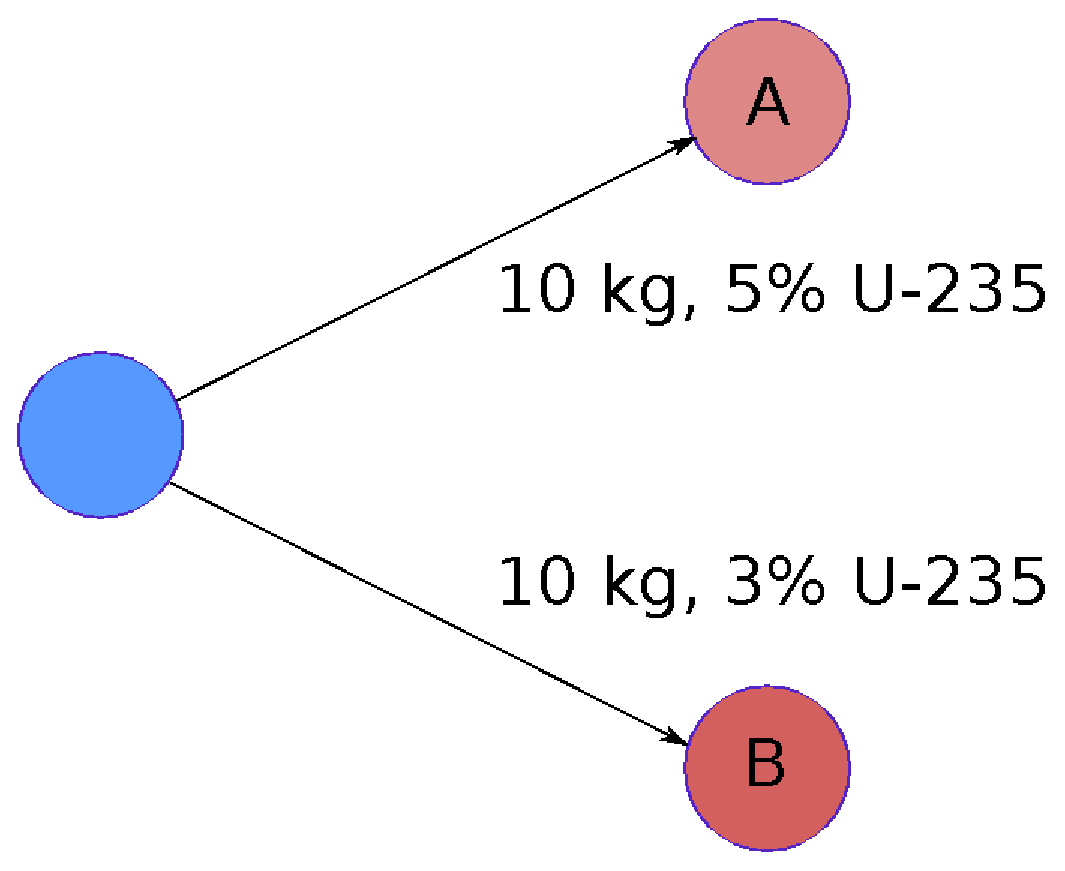
\includegraphics[height=3cm]{./images/enr.eps}
    \caption{Two Demands for Enriched Uranium}
  \end{figure}
  
  \begin{table} [h!]
    \begin{tabular}{|c|c|c|}
      \hline  
      Order & SWU & Nat'l U (kg) \\
      \hline  
      A & 71 & 112\\
      B & 34 & 64\\
      \hline  
    \end{tabular}
  \end{table}

\end{frame}

\begin{frame}[ctb!]
  \frametitle{Resource Exchange Generality}

  This proposal generalizes the exchange of resources in two steps:

  \begin{enumerate}
    \item Gather the information required to make a material flow decision
    \item Solve for material flow
  \end{enumerate}
\end{frame}

\begin{frame}[ctb!]
  \frametitle{Resource Exchange Information Gathering}

  Inspiration taken from Julka et. al. \cite{julka_agent-based_2002},

  \begin{itemize}
    \item fuel cycle is a supply chain
    \item individual facilities are agents
    \item petroleum industry also deals with material quality
  \end{itemize}
  
\end{frame}

\begin{frame}[ctb!]
  \frametitle{Resource Exchange: Request for Bids}
  \begin{figure}
    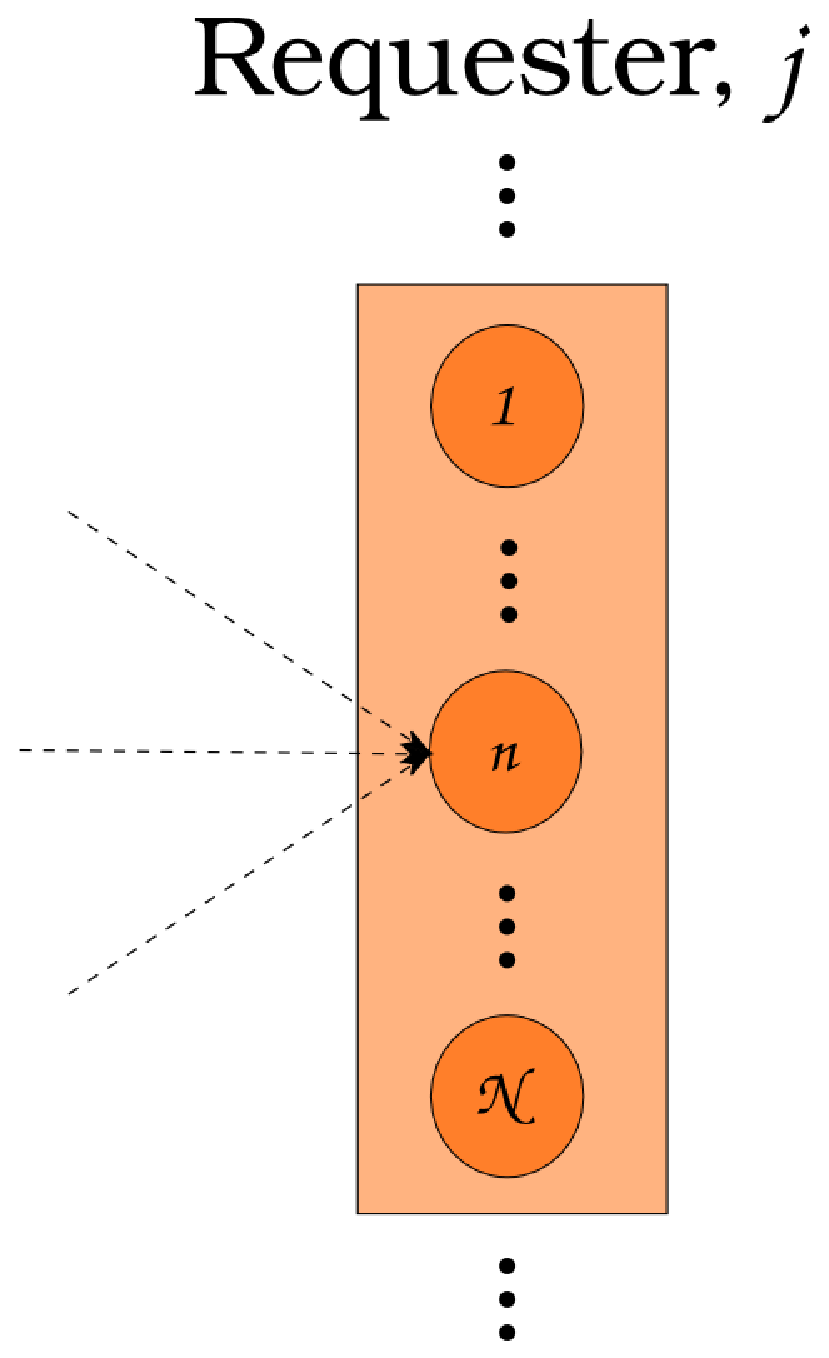
\includegraphics[height=5cm]{./images/requester.eps}
    \caption{Consumers define their demand for commodities during the Request
      for Bids (RFB) phase.}
  \end{figure}
\end{frame}

\begin{frame}[ctb!]
  \frametitle{Resource Exchange: Response to Request for Bids}
  \begin{figure}
    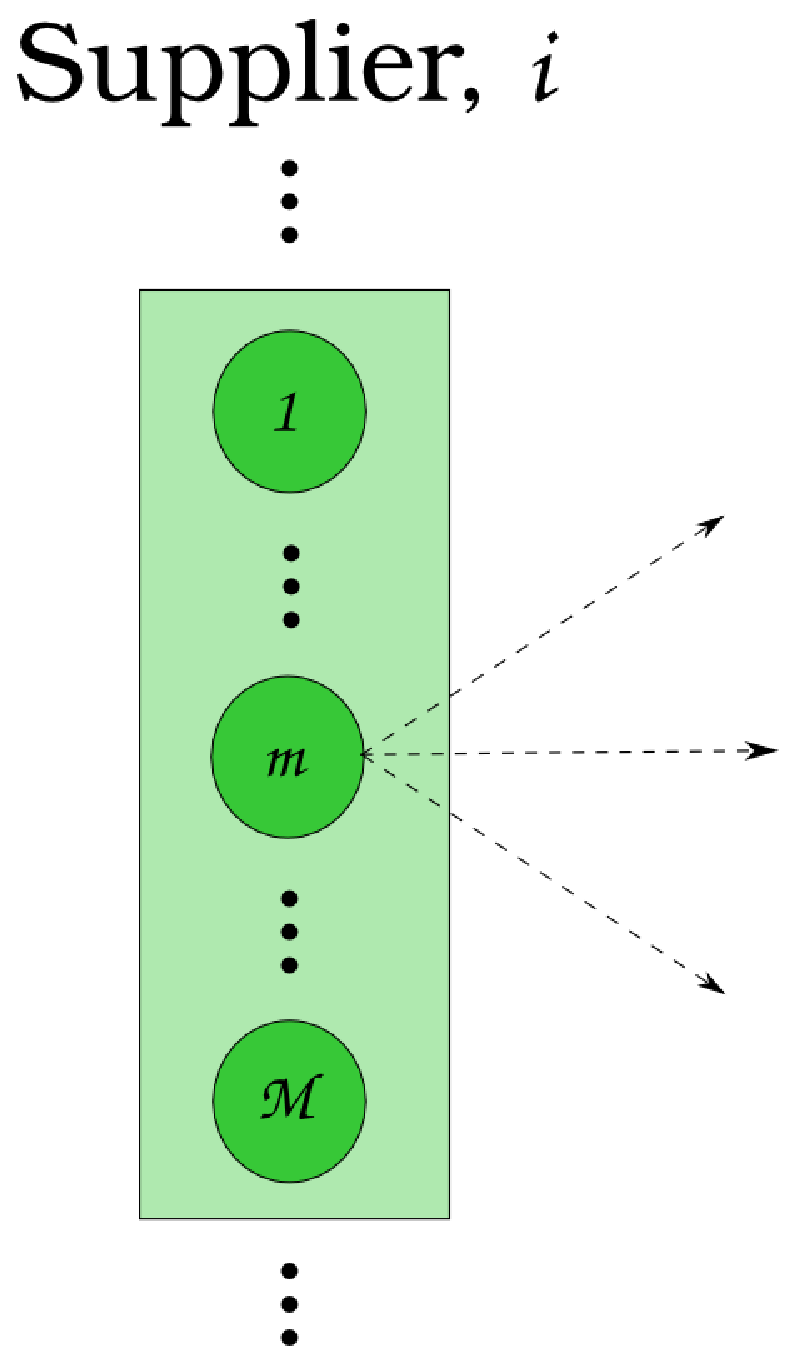
\includegraphics[height=5cm]{./images/supplier.eps}
    \caption{Suppliers respond to each request during the Response to Request
      for Bids (RRFB) phase.}
  \end{figure}
\end{frame}

\begin{frame}[ctb!]
  \frametitle{Resource Exchange: Preference Adjustment}
  \begin{figure}
    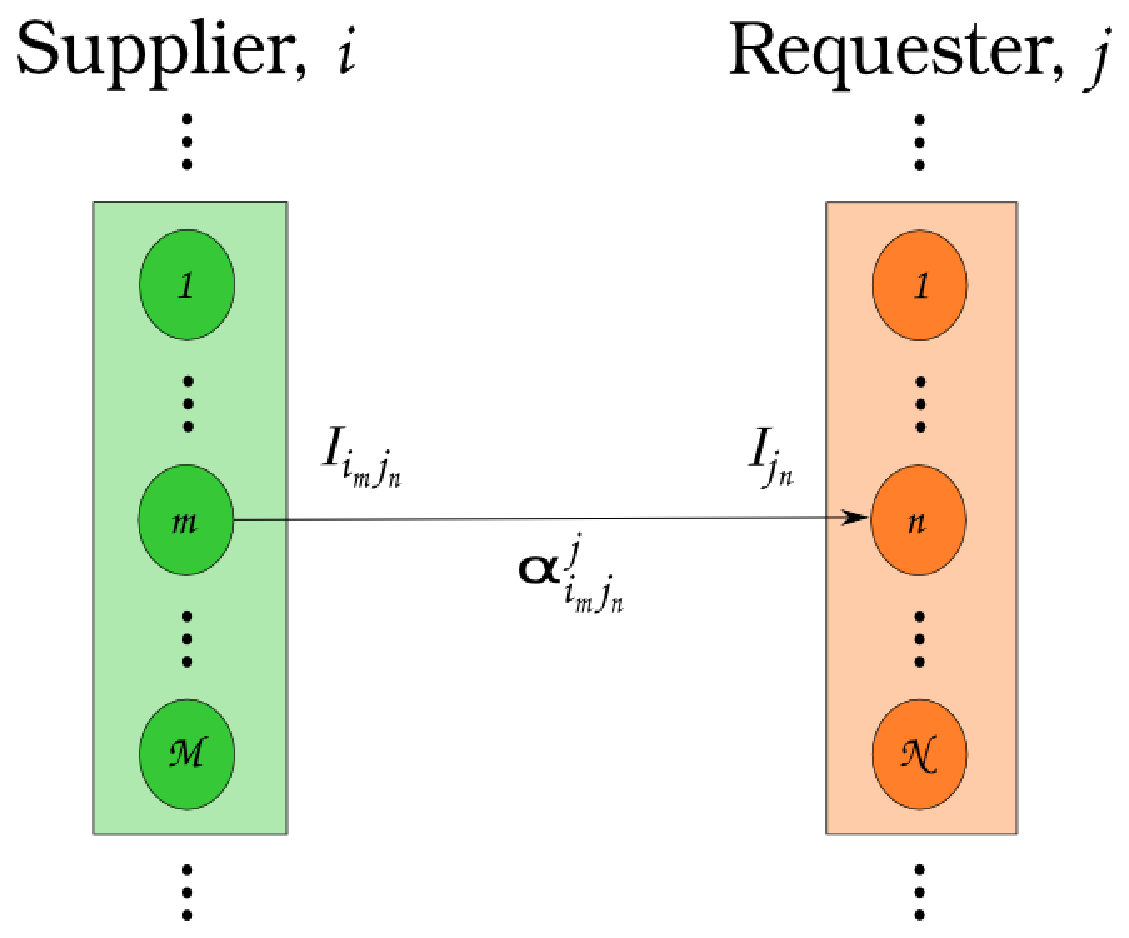
\includegraphics[height=4cm]{./images/supplier-requester.eps}
    \caption{Consumers adjust preferences based on Supplier-given information
      during the Preference Adjustment (PA) phase.}
  \end{figure}

  Managers of facilities (institutions, regions) are then allowed to perturb
  preferences.
\end{frame}

\begin{frame}[ctb!]
  \frametitle{Resource Exchange: Full Picture}
  \begin{figure}
    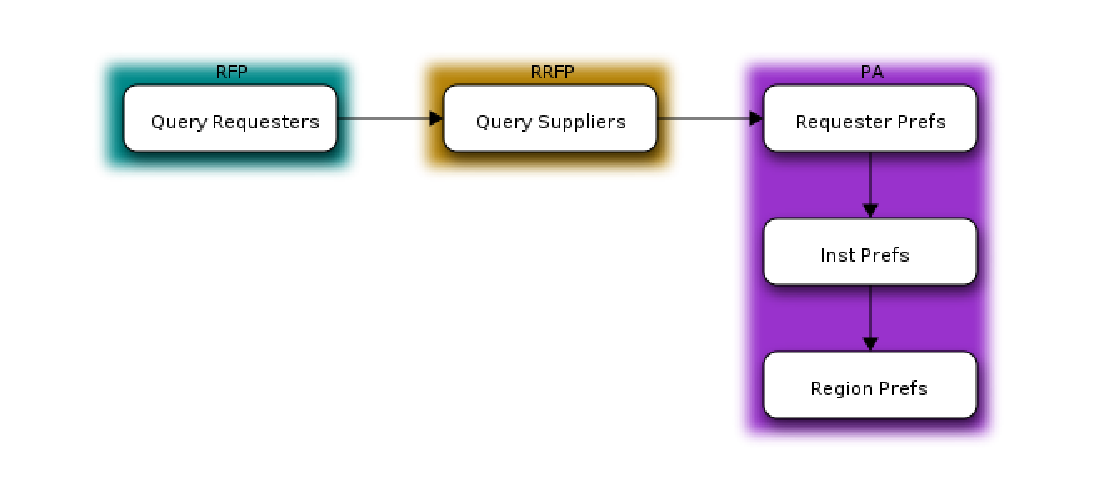
\includegraphics[height=5cm]{./images/exchange.eps}
    \caption{A flow chart of the information gathering phases.}
  \end{figure}
\end{frame}

\begin{frame}[ctb!]
  \frametitle{Resource Exchange Solution Mechanism}

  A Multicommodity Transportation Problem (MTP) formulation naturally fits the
  requirements of the simulation.

  \begin{itemize}
    \item supplier and consumer facilities
    \item discrete transfers of commodities
    \item demand can be met by multiple commodities
  \end{itemize}

  Departs from classic MTP, thus is called Generic Fuel Cycle Transportation
  Problem (GFCTP).
  
\end{frame}

\begin{frame}[ctb!]
  \frametitle{GFCTP - Overview}
  
  The Generic Fuel Cycle Transportation problem assumes the following:
  \begin{itemize}
    \item there is a set of suppliers, a set of requesters, a set of
      commodities, and a set of possible resource transfers, defining arcs
      between suppliers and requesters
    \item a cardinal preference ordering is defined over the set of possible
      resource transfers
    \item suppliers can be constrained both by resource quantities and qualities
    \item multiple commodity types may satisfy a consumer
  \end{itemize}

  A linear programming (LP) formulation and mixed integer-linear programming
  (MILP) formulation is proposed.

\end{frame}
  

\begin{frame}[ctb!]
  \frametitle{GFCTP - Nomenclature}

  Nomenclature used:
  \begin{itemize}
    \item set of commodities, $H$
    \item set of suppliers, $I$
    \item set of requesters, $J$
    \item flow, $x^h_{i,j}$
  \end{itemize}

\end{frame}

\begin{frame}[ctb!]
  \frametitle{GFCTP (LP) - Request Constraint}
  
  Requests
  \begin{itemize}
    \item can be met by multiple commodities, e.g., UOX and MOX
    \item are comprised of
      \begin{itemize}
        \item a quantity, $d_j$
        \item a set of commodities, $H_j$
      \end{itemize}
  \end{itemize}

  \begin{equation}
    \sum_{i \in I}\sum_{h \in H_{j}} x_{i,j}^{h} \geq d_{j}(H_{j})  \: \forall j \in J
  \end{equation}
  
  Feasibility can be guaranteed by using ``fake'' supplier with negative
  preference or infinite cost.

\end{frame}

\begin{frame}[ctb!]
  \frametitle{GFCTP (LP) - Supply Constraint - Example}

  Supply
  \begin{itemize}
    \item can have multiple possible constraints
    \item constraints can be functions of quality and quantity
  \end{itemize}

  E.g., an enrichment facility that provides the commodity enriched uranium (ER):
  \begin{itemize}
    \item A processing constraint, which has units of SWU
    \item An inventory constraint, which has units of kilograms of natural
      uranium (NU)
  \end{itemize}

\end{frame}

\begin{frame}[ctb!]
  \frametitle{GFCTP (LP) - Supply Constraint - Example}
  
  Given
  \begin{itemize}
    \item a requested enrichment level, $\varepsilon_j$
    \item a supply capacity, $s$
    \item a conversion function, $f$
  \end{itemize}

  Associated constraints are
  \begin{equation}
    \sum_{j \in J} f_{SWU}(\varepsilon_j) x_{i,j}^{EU} \leq s_{i,SWU} 
  \end{equation}

  \begin{equation}
    \sum_{j \in J} f_{NU}(\varepsilon_j) x_{i,j}^{EU} \leq s_{i,NU} 
  \end{equation}

  \pause

  These constraints are a function of the isotopic profile of the request, or
  \textit{quality}, $q_j$. More generally suppliers may have conversion
  functions, which are functions of the request quality,
  $\beta_{i,k}(q_{j}^{h})$.

\end{frame}

\begin{frame}[ctb!]
  \frametitle{GFCTP (LP) - Supply Constraint}

  Associated constraints are
  \begin{equation}
    \sum_{j \in J}\beta_{i,k}(q_{j}^{h}) x_{i,j}^{h} \leq s_{i,k} 
    \: \forall \: k \in K_{i}^{h},  
    \forall \: i \in I, \forall \: h \in H
  \end{equation}

  with notation defined as
  \begin{itemize}
    \item $h$ - a commodity
    \item $K_i^h$ - a set of constraints
    \item $s_{i,k}$ - a supply capacity
    \item $\beta_{i,k}(q_{j}^{h})$ - a conversion function
  \end{itemize}

\end{frame}

\begin{frame}[ctb!]
  \frametitle{GFCTP (LP) - Objective Function}

  Two options in proposed framework:
  \begin{enumerate}
    \item maximize preferences
    \item minimize cost
  \end{enumerate}

  Pros and cons:
  \begin{itemize}
    \item preferences are ``natural'' fit
    \item economics is a future concern
    \item cost minimization requires a translation function
  \end{itemize}

\end{frame}

\begin{frame}[ctb!]
  \frametitle{GFCTP (LP) - Objective Function}

  Assuming there is such a function, $f$, i.e.,
  \begin{equation}
    f : \alpha_{i,j}(h) \to c_{i,j}^{h}
  \end{equation}

  The the objective function is
  \begin{equation}
    \min \sum_{h \in H}\sum_{i \in I}\sum_{j \in J}c_{i,j}^{h} x_{i,j}^{h} 
  \end{equation}

\end{frame}

\begin{frame}[ctb!]
  \frametitle{GFCTP (LP) - Formulation} 

  With the normal non-negative flow constraint, the full GFCTP formulation is:
  
  %%%
  \begin{subequations}\label{eqs:GFCTP-LP}
    \begin{align}
      %%
      \min_{z} \:\: & 
      z = \sum_{h \in H}\sum_{i \in I}\sum_{j \in J}c_{i,j}^{h} x_{i,j}^{h} 
      & \label{eqs:GFCTP-LP_obj} \\
      %%
      \text{s.t.} \:\: &
      \sum_{j \in J}\beta_{i,k}(q_{j}^{h}) x_{i,j}^{h} \leq s_{i,k} 
      &
      \: \forall \: k \in K_{i}^{h},  
      \forall \: i \in I, \forall \: h \in H \label{eqs:GFCTP-LP_sup} \\
      %%
      &
      \sum_{i \in I}\sum_{h \in H_{j}} x_{i,j}^{h} \geq d_{j}(H_{j}) 
      & 
      \forall \: j \in J \label{eqs:GFCTP-LP_dem} \\
      %%
      &
      x^h_{i,j} \geq 0
      &
      \forall \: x \in X \label{eqs:GFCTP-LP_x}
      %%
    \end{align}
  \end{subequations}
  %%% 
\end{frame}

\begin{frame}[ctb!]
  \frametitle{GFCTP (LP) - Comments} 
  
  Issues with LP formulation:
  \begin{enumerate}
    \item orders can be split
    \item orders can be satisfied by multiple suppliers
  \end{enumerate}

  Consider a thermal reactor's order constraint for UOX and MOX under the LP
  framework:
  \begin{equation}
    \sum_{i \in I} x_{i}^{MOX} + x_{i}^{UOX} \geq d(\{MOX,UOX\})
  \end{equation} 

  Given a solution, $x^{MOX}$, and $x^{UOX}$, the following values are possible:
  \begin{equation}
    x^{MOX} \in [0, d(\{MOX,UOX\})], \: x^{UOX} \in [0, d(\{MOX,UOX\})]
  \end{equation} 

\end{frame}

\begin{frame}[ctb!]
  \frametitle{GFCTP (MILP) - Overview}

  Split consumers into two groups:
  \begin{enumerate}
    \item those that require \textit{exclusive} orders
    \item those allow \textit{partial} orders
  \end{enumerate}

  \begin{equation}\label{eqs:consumer-union}
    J = J_{p} \cup J_{e}
  \end{equation}

  Introduce a binary variable, $y_{i,j}^{h}$.  
  \begin{itemize}
    \item 1 if consumer $j$ is sent commodity $h$ by supplier $i$
    \item restrict sum of variables for consumer $j$ to 1
  \end{itemize}

  \begin{equation}
    \sum_{h \in H_j}\sum_{i \in I}  = 1
     \: \forall \: j \in J_{e}
  \end{equation}
  
\end{frame}

\begin{frame}[ctb!]
  \frametitle{GFCTP (MILP) - Request Constraint} 

  There are now two requests constraints, for each family of requests:

  \begin{equation}
    \sum_{i \in I}\sum_{h \in H_{j}} x_{i,j}^{h} \geq d_{j}(H_{j})
     \: \forall \: j \in J_{p}
  \end{equation}
  
  \begin{equation}    
    \sum_{i \in I}\sum_{h \in H_{j}} y_{i,j}^{h} \tilde{x}_{j}^{h} \geq d_{j}(H_{j}) 
     \: \forall \: j \in J_{e}
  \end{equation}

  The combination $y_{i,j}^{h} \tilde{x}_{j}^{h}$ is equivalent to the flow of
  commodity $h$ from supplier $i$ to requester $j$, $x^h_{i,j}$.
\end{frame}

\begin{frame}[ctb!]
  \frametitle{GFCTP (MILP) - Supply Constraint} 

  Supply constraints also incorporate to two possible flows of material out of a
  supplier:
  
  \begin{equation}    
    \sum_{j \in J_{p}}\beta_{i,k}(q_{j}^{h}) x_{i,j}^{h}
    + \sum_{j \in J_{e}}\beta_{i,k}(q_{j}^{h}) y_{i,j}^{h} \tilde{x}_{j}^{h} \leq s_{i,k}^{h}
     \: \forall \: i \in I, \: \forall \: k \in K_{i}^{h}, \forall \: {h \in H}
  \end{equation}
  
\end{frame}

\begin{frame}[ctb!]
  \frametitle{GFCTP (MILP) - Formulation} 
  
  With a similar treatment of the objective function, the full formulation is:
  
  \begin{subequations}\label{eqs:GFCTP-E}
    \begin{align}
      %%
      \label{eq:GRCTP-E_obj}
      \min_{z} \:\: 
      & 
      z = \sum_{h \in H}\sum_{i \in I}\sum_{j \in J_{p}}c_{i,j}^{h} x_{i,j}^{h} 
      + \sum_{h \in H}\sum_{i \in I}\sum_{j \in J_{e}}c_{i,j}^{h} y_{i,j}^{h} \tilde{x}_{j}^{h}
      && \\
      %%
      \label{eq:GRCTP-E_sup}
      &
      \text{s.t.} \:\: 
      \sum_{j \in J_{p}}\beta_{i,k}(q_{j}^{h}) x_{i,j}^{h}
      + \sum_{j \in J_{e}}\beta_{i,k}(q_{j}^{h}) y_{i,j}^{h} \tilde{x}_{j}^{h} \leq s_{i,k}^{h} \nonumber \\
      &
      \qquad\qquad\qquad\qquad
      \forall \: i \in I, \: \forall \: k \in K_{i}^{h}, \forall \: {h \in H}\\
      %%
      \label{eq:GRCTP-E_dem_p}
      &
      \sum_{i \in I}\sum_{h \in H_{j}} x_{i,j}^{h} \geq d_{j}(H_{j})
      &
      \forall \: j \in J_{p} &\\
      %%
      \label{eq:GRCTP-E_dem_e}
      &
      \sum_{i \in I}\sum_{h \in H_{j}} y_{i,j}^{h} \tilde{x}_{j}^{h} \geq d_{j}(H_{j}) 
      &
      \forall \: j \in J_{e}  &\\
      %%
      \label{eq:GRCTP-E_sumy}
      &
      \sum_{h \in H}\sum_{i \in I} y_{i,j}^{h} = 1
      &
      \forall \: j \in J_{e}  &\\
      %%
      \label{eq:GRCTP-E_x}
      &
      x_{i,j}^{h} \geq 0
      &
      \forall \: x \in X  &\\
      %%
      \label{eq:GRCTP-E_y}
      &
      y_{i,j}^{h} \in \{0,1\}
      &
      \forall \: y \in Y &
      %%
    \end{align}
  \end{subequations}

\end{frame}

\begin{frame}[ctb!]
  \frametitle{Recipe Approximation Problem - Set Up} 

  Originally posed in a slightly different form by Oliver
  \cite{oliver_geniusv2:_2009}, the RAP assumes:
  \begin{enumerate}
    \item a recycled fuel fabrication facility has a set of barrels of separated
      material
    \item each barrel is a homogeneous mixture of its isotopics
    \item barrels have a mass, $m_b$, and isotopic profile, $I_b$
    \item there are a set of target recipes
    \item target recipes have a mass, $m_t$, and isotopic profile, $I_t$
  \end{enumerate}

  Goal: Match the recipes as ``closely'' as possible.
\end{frame}

\begin{frame}[ctb!]
  \frametitle{Recipe Approximation Problem - Set Up} 
  \begin{figure}
    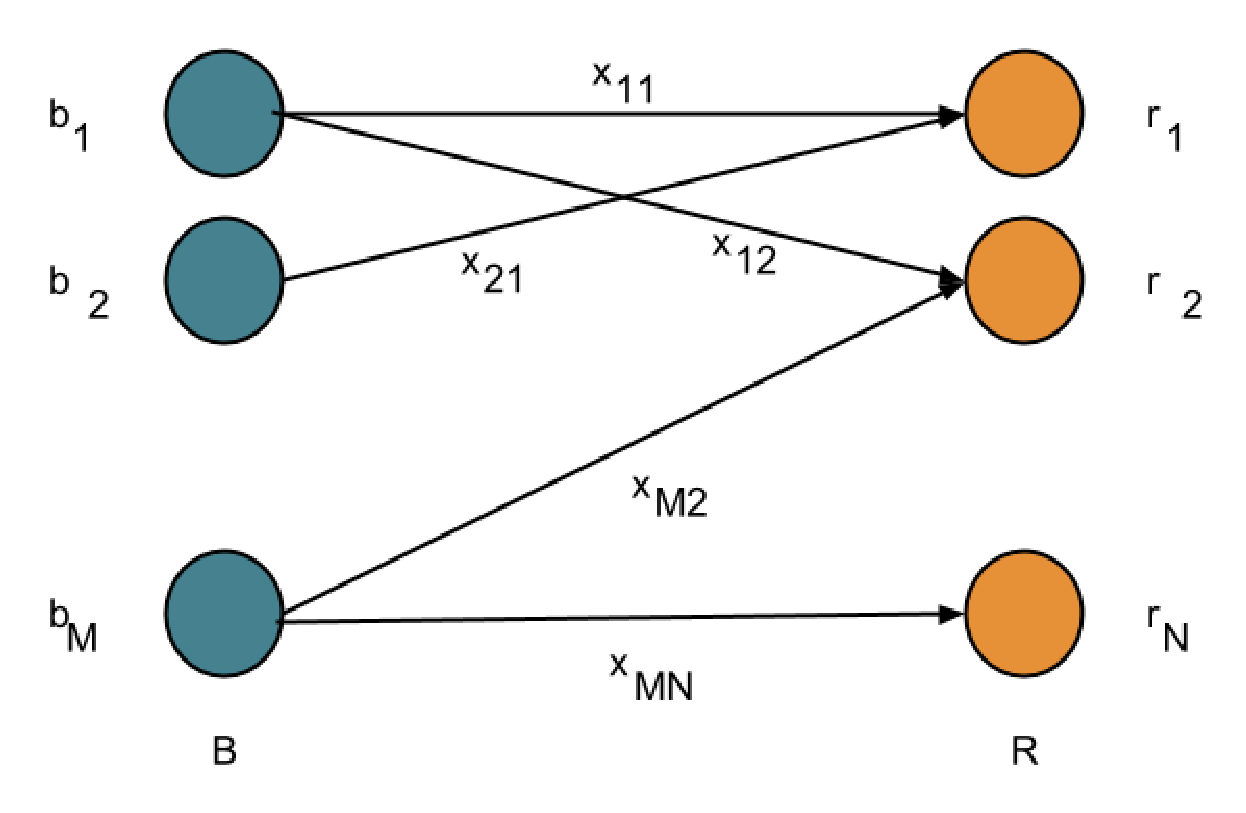
\includegraphics[height=5cm]{./images/rap.eps}
    \caption{A pictorial example of the Recipe Approximation Problem.}
  \end{figure}
\end{frame}

\begin{frame}[ctb!]
  \frametitle{Recipe Approximation Problem - Set Up} 

  An $\ell_1$ norm approximation formulation is used.\vspace{0.2cm}
  
  The objective function and constraints are comprised of properties of the
  determined solution.\vspace{0.2cm}

  The constraint properties are required to be met within some error, whereas
  the residual of the objective property is minimized.
\end{frame}

\begin{frame}[ctb!]
  \frametitle{Recipe Approximation Problem - Objective}

  In the current formulation, matching the target recipe is the objective.
  
  The residual is defined as
  \begin{equation}\label{eqs:residual}
    \vec{y_{t}} = \left| M \cdot \vec{x_{t}}  - m_t \vec{I_{t}} \right|.
  \end{equation}

  Given
  \begin{itemize}
    \item a barrel mass matrix $M$, i.e., $I_b * m_b$ for each barrel
    \item a feasible solution for a target recipe, $x_t$
  \end{itemize}

  The sum of residuals is minimized, using a weighting factor, $c_t$,
  \begin{equation}\label{rap-obj}
    \min_{z} \:\: z = \sum_{t \in T} \vec{c_{t}}^{\top} \cdot \vec{y_{t}}
  \end{equation}
\end{frame}

\begin{frame}[ctb!]
  \frametitle{Recipe Approximation Problem - Objective Weights}

  Issues with strictly matching recipes include:
  \begin{enumerate}
    \item presence of contaminants
    \item relative importance of fertile vs. fissile isotopes
  \end{enumerate}

  \vspace{0.2cm}

  A weighting factor is used to normalize contributions to the objective
  function:
  \begin{equation}\label{eqs:weights}
    c_{i,t} = 
    \begin{cases}
      \frac{1}{m_{i,t}} & \text{if } i \in I_{t} \\
      \frac{1}{m_{t}}   & \text{if } i \not\in I_{t}
    \end{cases}
  \end{equation}  
\end{frame}

\begin{frame}[ctb!]
  \frametitle{Recipe Approximation Problem - Mass Constraint}

  The mass differential is constrainted
  \begin{itemize}
    \item the solution should have approximately the same mass as the target
    \item a maximum violation, $\epsilon_{m}$, is provided
  \end{itemize}
  
  \begin{equation}\label{eqs:mass-constraint-simple}
    \epsilon_{m} \geq \left| m_{x_t} - m_{t} \right|.
  \end{equation}
\end{frame}

\begin{frame}[ctb!]
  \frametitle{Recipe Approximation Problem - Neutronics Constraint}

  A neutronics parameter is constrainted
  \begin{itemize}
    \item the solution should behave similar neutronically to the target
    \item neutron reproduction factor, $\eta$, is chosen
    \item $\eta$ is a function solely of the recipe, not reactor geometry, etc.
  \end{itemize}
\end{frame}

\begin{frame}[ctb!]
  \frametitle{Recipe Approximation Problem - Neutronics Constraint}

  $\eta$ is defined for a homogeneous material as:
  \begin{equation}
    \label{eqs:eta_micro}
    \eta_{t} = \frac{\sum_{i \in I_t} \nu^{i} \sigma_{f}^{i} N^{i}} {\sum_{i
        \in I_t} \sigma_{a}^{i} N^{i}},
  \end{equation}

  with physical constants:
  \begin{itemize}
    \item $\nu^{i}$ - the average number of neutrons produced by fission of isotope $i$
    \item $\sigma_{f}^{i}$ - the microscopic fission cross section for isotope $i$
    \item $\sigma_{a}^{i}$ - the microscopic absorption cross section for isotope $i$
    \item $N^i$ - the number density of isotope $i$
  \end{itemize}
\end{frame}

\begin{frame}[ctb!]
  \frametitle{Recipe Approximation Problem - Neutronics Constraint}

  From the perspective of mixing of barrels, one can define the reproduction
  factor of a proposed solution as:

  \begin{equation}
    \label{eqs:eta_simple}
    \eta_{x_t} = \frac{\sum_{b \in B} \eta_{b}^{+} x_{b, t}}
        {\sum_{b \in B} \eta_{b}^{-} x_{b, t}}
  \end{equation}

  Where $\eta_b^+$ and $\eta_b^-$ are defined as:

  \begin{equation}
    \label{eqs:eta_+}
    \eta_{b}^{+} \equiv \sum_{i \in I_{b}} \nu^{i} \sigma_{f}^{i} N_{b}^{i}
  \end{equation}

  \begin{equation}
    \label{eqs:eta_-}
    \eta_{b}^{-} \equiv \sum_{i \in I_{b}} \sigma_{a}^{i} N_{b}^{i}
  \end{equation}
  
\end{frame}

\begin{frame}[ctb!]
  \frametitle{Recipe Approximation Problem - Neutronics Constraint} 

  This separation allows one to write the neutronics constraint, given a maximum
  possible violation, $\epsilon_{\eta}$, as:

  \begin{equation}
    \label{eqs:eta_linear}
    \epsilon_{\eta} \sum_{b \in B} \eta_{b}^{-} x_{b,t} \geq
    \left| \sum_{b \in B} \eta_{b}^{+} x_{b,t}
    - \eta_{t} \sum_{b \in B} \eta_{b}^{-} x_{b,t} \right|
  \end{equation}  
\end{frame}

\begin{frame}[ctb!]
  \frametitle{Recipe Approximation Problem - Formulation}

  The full formulation for the RAP is then:
  \fontsize{7pt}{\baselineskip}\selectfont
  %%% 
  \begin{subequations}\label{eqs:rap}
    \begin{align}
      %%
      \min_{z} \:\: & 
      z = \sum_{t \in t} \vec{c_{t}}^{\top} \cdot \vec{y_{t}}
      & \label{eqs:rap_obj} \\
      %%
      \text{s.t.} \:\: &
      \vec{y_{t}} = \left| M \cdot \vec{x_{t}}  - m_t \vec{I_{t}} \right|
      &
      \forall t \in T \label{eqs:rap_iso} \\
      %%
      &
      \epsilon_{m} \geq \left| \sum_{b \in B} m_{b} x_{b, t} - m_{t} \right|
      & 
      \forall t \in T \label{eqs:rap_mass} \\
      %%
      &
      \epsilon_{\eta} \sum_{b \in B} \eta_{b}^{-} x_{b, t} \geq 
      \left| \sum_{b \in B} \eta_{b}^{+} x_{b, t} - 
      \eta_{t} \sum_{b \in B} \eta_{b}^{-} x_{b, t} \right|
      & 
      \forall t \in T \label{eqs:rap_eta} \\
      &
      \sum_{t \in T} x_{b, t} \leq 1
      & 
      \forall b \in B \label{eqs:rap_conserv} \\
      &
      x_{b, t} \in \left[ 0, 1 \right]
      & 
      \forall b \in B, \forall t \in T  \label{eqs:rap_x}
      %%
    \end{align}
  \end{subequations}
  %%% 
\end{frame}

\begin{frame}[ctb!]
  \frametitle{Recipe Approximation Problem - Research Questions} 

  Four primary research questions exist:

  \begin{enumerate}
    \item Does barrel size affect the accuracy of matches?
    \item Is isotopic ``closeness'' or neutronics parameter ``closeness'' the
      better objective function value?
    \item How to delineate between fast and thermal recipes?
    \item Are additional neutronics constraints helpful?
  \end{enumerate}
\end{frame}

\begin{frame}[ctb!]
  \frametitle{Next Steps} 
  
  \begin{itemize}
    \item all work will be done in the
      \href{github.com/cyclus/cyclus}{\Cyclus} code base, incorporating
      continuous integration and unit testing
    \item the \Cyclus team has identified the one and two-tier fuel cycles
      proposed in the recent Dynamic Systems Analysis Report for Nuclear Fuel
      Recycle (DSARR) \cite{dixon_dynamic_2008} as targets for
      development
    \item \Cyclus requires additional capability for modeling instances of
      multiple commodity supply/demand
    \item the proposed Information Gathering mechanism can supply this capability
      and provide downstream flexibility for future work
  \end{itemize}
\end{frame}

\begin{frame}[ctb!]
  \frametitle{Next Steps} 

  \begin{itemize}
    \item the LP formulation of the GFCTP will be implemented for this simple
      case
    \item the DSAR scenario will be extended to include multiple regions to
      provide a proof-of-principle example of preference-based material flow
    \item the MILP formulation for the GFCTP will then be implemented
    \item comparisons in run time and output will be observed, and, depending on
      outcomes, acceleration methods, such as cutting planes and preprocessing,
      will be investigated
    \item COIN-OR\cite{lougee_common_2003} open source libraries will be used
  \end{itemize}
\end{frame}

\begin{frame}[ctb!]
  \frametitle{Next Steps} 
  
  \begin{itemize}
    \item initially, a ``naive'' advanced fabrication facility will be used
    \item the RAP will be implemented 
    \item comparisons will be made with current approaches (e.g. COSI's equivalence method)
    \item simulation-level effects will be investigated (e.g., barrel size)
    \item again, COIN-OR open source libraries will be used
  \end{itemize}
\end{frame}

\section{Acknowledgements}
\include{acknowledgements}

%||||---------------
\begin{frame}[allowframebreaks]
  \frametitle{References}
  \bibliographystyle{plain}
  \bibliography{main}
\end{frame}
%---------------||||




\end{document}
